For this study, we employ a simple Dansgaard-Johnsen-type ice flow model \citep{schwander2001}. We do not include a separate term for basal melting, which is likely occurring or has occurred at this site as liquid water was observed at the bed during drilling \citep{gow1968}. The inclusion of a melt condition is expected to increase accumulation rate estimates to account for ice loss at the bedrock interface. We exclude basal melting because we lack estimates of basal melt rate over time. However, this method could be adapted to incorporate a more sophisticated flow model with additional parameters such as a non-zero melt rate. 

%Our results also demonstrate the importance of our choice of priors, particularly in accumulation rate parameters at depth. We chose uninformative priors due to our lack of knowledge about local accumulation rates at the Byrd ice core site prior to the LGM. However, more informed priors could be assumed to perhaps better constrain accumulation rate estimates at the bottom of the ice column. 

%Our method is sensitive to correlations between parameter estimates, consistent with expectations that parameters may covary with depth. 

To estimate the ice flow and accumulation rate parameters in our model, we must assume the effective number of degrees of freedom, $k_e$,  because it is not known. The number of degrees of freedom helps determine the significance of errors between our model and the volcanic chronology. Because we use these errors as a measure of uncertainty through paramater $S$, $k_e$ has a direct role in determining the uncertainty in age estimates. Estimates of $k_e$ using our ice flow model to represent the effect of uncertainites in ice flow parameters and accumulation rates on age estimates varied depending on assumptions about these model parameters. Given this variation and the potentially circular logic in this method, we instead choose $k_e = \frac{j}{2}$ = 30.5, which assumes there are strong correlations among age solutions. This is reasonable because we expect errors in age and depth are related within the ice column. 
%The solution uncertainty is affected by the value of $k_e$ as shown by the sensitivity of our results to our choice of $k_e$ in Figure~\ref{fig:ke}. 
%However, we find that our choice of $k_e$ does not significantly impact the mean estimates of age or depth for our radar reflectors. %In lieu of independent information about an appropriate value of $k_e$, we choose to assume $k_e = \frac{J}{2} = 30.5$ because mixing of the accumulation rate parameters is strong and the rate at which the algorithm finds solutions is reasonable. 
%For our age likelihood and estimation of $S$, we assume $k_e$ = 50\% of the number of volcanic data points. 
As shown in Figure~\ref{fig:ke}, this choice does not affect mean estimates of reflector age and depth, but it does have some affect on the uncertainty associated with them. 
% Our result could therefore be improved through more work toward an independent determination of an appropriate value for $k_e$. 

\begin{figure*}
\begin{center}
%\centering
\makebox[\textwidth][c]{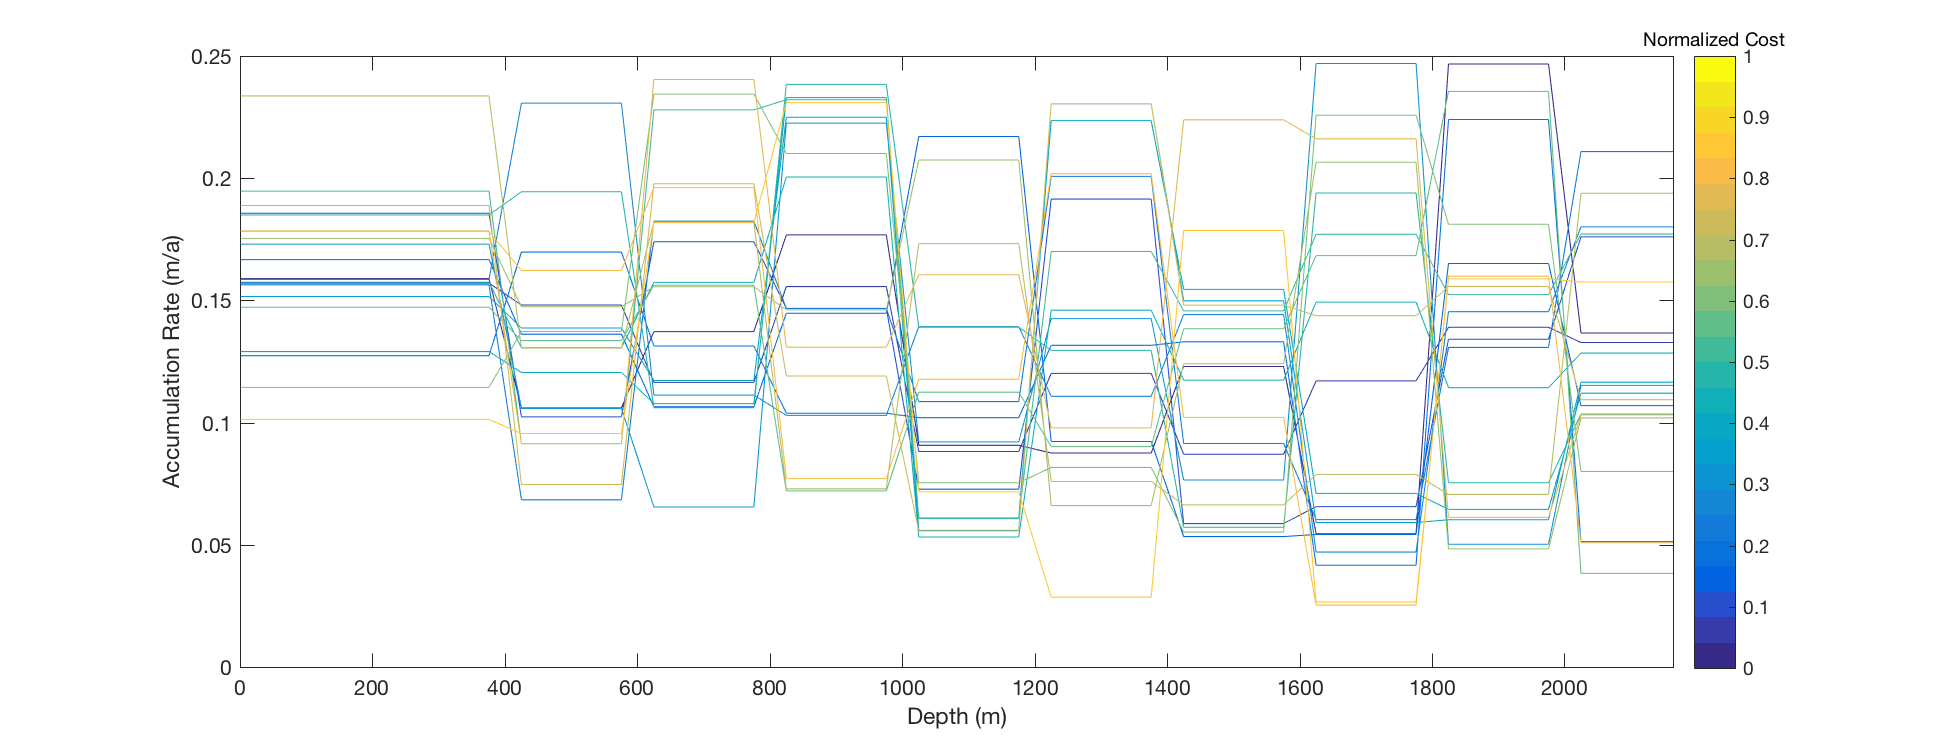
\includegraphics[scale=0.5]{/Users/gail/Documents/Research/Projects/age-depth-firninvert/analysis/figures/keCompare}}
%\captionsetup{width=.9\textwidth}
\caption{Comparison of reflector age for different degrees of freedom, $k_e$, relative to the number of volcanic data points, $j=61$. The choice of $k_e$ has an effect on uncertainty in reflector age estimates, but does not greatly impact mean estimates. }
\end{center}
\label{fig:ke}
\end{figure*}


%All such dating efforts should agree at multiple ice core locations as in \citet{cavitte2016}. We see agreement between our mean estimated reflector ages at the Byrd ice core and those observed at the WAIS Divide ice core, but 
Uncertainties in our estimates of radar reflector depth are significant compared to those derived from the age determination alone. These relatively large uncertainties from the radar can be attributed to radar range precision in the determination of reflector depths. This precision is a function of the signal-to-noise ratio (SNR) of the radar reflection and bandwidth of the radar system used to obtain the reflections \citep{cavitte2016}. Increasing SNR would improve range precision and reduce uncertainty, however our method already selects for high SNR in analyzing only the brightest reflectors in the ice column. As a result, we expect the data do not support improving precision in this way. Increasing bandwidth (15 MHz for the HiCARS radar system) would also improve the radar range precision, however this is technically challenging for modern airborne radar systems because antenna tuning is difficult for bandwidths greater than 25\% of the center frequency (60 MHz for the HiCARS system). Ground penetrating radar systems can have higher bandwidth, but are more limited in their spatial coverage. Further, while higher resolution can be obtained by increasing bandwidth and center frequency, penetration through the ice declines and reflections become increasingly discontinuous with increasing bandwidth \citep{cavitte2016}.





 %estimates tend younger than those at the Byrd ice core site. It is unclear why this is the case, though it may be attributable to additional missing uncertainties in drilling of the Byrd ice core. Through use of local density measurements at the WAIS Divide ice core, we exclude differences in firn thickness to account for this discrepancy. %However, as an early deep-drilling effort, less sophisticated technology used at the Byrd ice core may have led to more deviations in the drilling direction than reported, for example. Deviations from vertical may lead to a longer core sample than the true ice thickness and may skew the reported volcanic chronology (as measured from the ice core) to be older than it really is. 

